% design and analysis
%
% DESIGN AND ANALYSIS: Objective of the study, data source, statistical model/tools/methodology, 
% validity of the assumptions if any, results of the study (graphs, tables will go here),
% results discussion, (interpretations/consclusions/inferences)
%
%----------------------------------------------------------------------------------------
%	PACKAGES AND OTHER DOCUMENT CONFIGURATIONS
%----------------------------------------------------------------------------------------
% none


\section{Design and Analysis}
To best model the dichotomous response variable, Y\textunderscore HighGradeCancer, in the Prostate Cancer case study, I will employ a multiple logistic regression model, where 1 indicates high grade cancer and 0 indicates not high grade cancer. \par
In statistics, if \(\pi = f(x)\) is a probability then \(\frac{\pi}{1-\pi}\) is the corresponding \textit{odds}, and the \textbf{logit} of the probability is the logarithm of the odds:
\begin{equation}
	logit(\pi) = log(\frac{\pi}{1-\pi})
\end{equation}

Now, simple logistic regression means assuming that \(\pi(x)\) is related to \(\beta_0 + \beta_1x\) (the \textit{logit response function}) by the logit function. By equating \(logit(\pi)\) to the logit response function, we understand that the logarithm of the odds is a linear function of the predictor. In particular, the slope parameter \(\beta_1\) is the change in the log odds associated with a one-unit increase in \textit{x}. This implies that the odds itself changes by the multiplicative factor \(e^{\beta_1}\) when \textit{x} increases by 1 unit.

\begin{equation}
	log(\frac{\pi}{1-\pi}) = \beta_0 + \beta_1x
\end{equation}

From here, straightforward algebra will then show the Simple Linear Regression Model:

\begin{equation}
	E[Y] = \pi(x) = \frac{e^{\beta_0 + \beta_1x}}{1+e^{\beta_0 + \beta_1x}}
\end{equation}

Next, this simple logistic regression model is easily extended to more than one predictor variable by inclusion of the following two vectors, in matrix notation:

\[
	\boldsymbol{\beta} = 
	\begin{bmatrix}
		\beta_0 \\ \beta_1 \\ \vdots \\ \beta_{p-1}
	\end{bmatrix} \quad
	\textbf{X} = 
	\begin{bmatrix}
		1 \\ X_1 \\ X_2 \\ \vdots \\ X_{p-1}
	\end{bmatrix} 
\]

With this notation, the simple logistic response function (Eqn. 3) extends to the multiple logistic response function as follows:

\begin{equation}
	E[Y] = \pi(\textbf{X}) = \frac{exp(\textbf{X}'\boldsymbol{\beta})}{1+exp(\textbf{X}'\boldsymbol{\beta})}
\end{equation}

Fitting the logistic regression to the sample data requires that the parameters \(\beta_0\), \(\beta_1\),\(\cdots\), \(\beta_{p-1}\) be estimated. This will be done using the maximum likelihood technique provided within the statistical packages of both \textbf{R} and \textit{Python}.

\subsection{Data Transformations and Standardization}
Variable transformation is an important technique to create robust models using logistic regression, and the appropriate transformations on continuous variables are necessary to optimize the model predictiveness. Because the predictors are linear in the log of the odds, it is often helpful to transform the continuous variables to create a more linear relationship. \par 
The raw data collected contained several predictors with high skewness values. A few concerning features were determined to be PSA Level (skewness = 4.39), Cancer Volume (skewness = 2.18), and Weight (skewness = 7.46). As a prepossessing step to reduce skewness, I elected to transform these continuous predictor variables using the log-transformation, and standardize \textit{all} the data on top of that. The standardization step was used to normalize the data, and did not affect any underlying distributions among the predictor variables. \par
The finalized data skewness is summarized directly below in Figure 1. 

\begin{figure}[H]
	\centering
	\includegraphics[scale=0.9]{final_skewness}
	\caption{Finalized Skewness Values of Transformed Predictor Variables.}
\end{figure}

Additionally, I've included the histogram of PSA Level vs. Cancer Volume in Figure 2 - a helpful visual for the two predictors which carried the most significance through much of my analysis, as we soon shall see. Notice how the distributions exhibit no notable skewness, are quite symmetrical, and are centered on zero.

\begin{figure}[H]
	\centering
	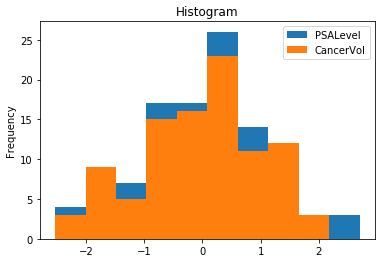
\includegraphics{psalevel_cancervol_skewness}
	\caption{Finalized PSALevel vs. CancerVol Histogram.}
\end{figure}

\subsection{Model Selection}
The data of 97 individual men in the Prostate Cancer sample was split at 80\% for train (model-building) and test (validation) sets. The training set is a random 76 observations and was used for fitting the model, and the remaining 21 cases were saved to serve as a validation data set. Figure 3 in columns 1-8 contains the variables, and shows a portion of the finalized and processed training data. \par
The primary purpose of the study was to asses the strength of the association between each of the predictor variables with the response variable, the predictable nature of PSA Level, and the probability of a man having been diagnosed with high grade prostate cancer over low grade.

\begin{figure}[H]
	\centering
	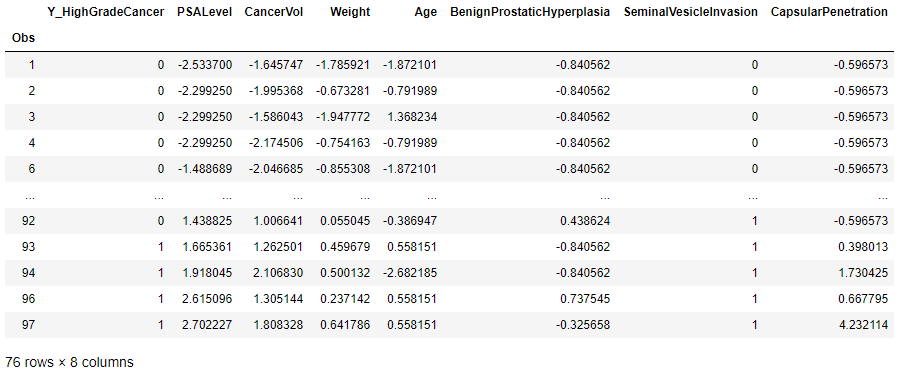
\includegraphics[scale=0.7]{train_data_python}
	\caption{Portion of Processed Model-Building Data Set - \textit{Python} Dataframe.}
\end{figure}

\subsubsection{Best Subsets Procedure}
The procedure outlined here will help identify a group of subset models that give the best values of a specified criterion. This technique has been developed by time-saving algorithms which can find the most promising models, without having to evaluate all \(2^{p-1}\) candidates. The use of the best subset procedure is based on the \textit{AIC\textsubscript{p}} criteria, where promising models will yield a relatively small value. \par
The minimized \textit{AIC\textsubscript{p}} stepwise output given by \textbf{R} is provided in Figure 4 below.

\begin{figure}[H]
	\centering
	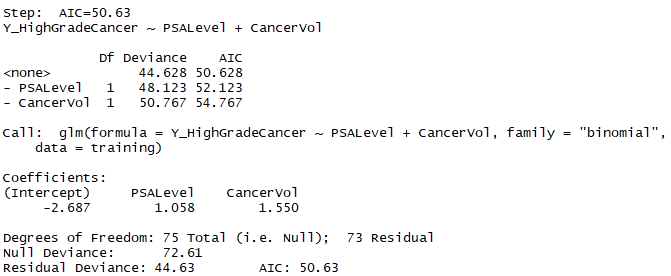
\includegraphics[scale=0.9]{best_subset}
	\caption{Full Linear Model  \textit{AIC\textsubscript{p}} Best Subset Results - \textbf{R} Output.}
\end{figure}

In this procedure, I instructed \textbf{R} to iterate "backwards" through all 7 predictor variables and it was determined \textit{AIC\textsubscript{p}} was minimized for \(p=3\). In particular, the results reveal that the best two-predictor model for this criteria is based on \textit{PSA Level} and \textit{Cancer Volume}. The \textit{AIC\textsubscript{p}} was minimized to 50.63, with a Null Deviance equal to 72.61 and Residual Deviance equal to 44.63. 

\subsubsection{Model Fitting}
A first-order multiple logistic regression model with two predictor variables was considered to be reasonable by \S4.2.1: 

\begin{equation}
\pi(\textbf{X}) = \frac{exp(\textbf{X}'\boldsymbol{\beta})}{1+exp(\textbf{X}'\boldsymbol{\beta})} = [1+exp(-\textbf{X}'\boldsymbol{\beta})]^{-1}
\end{equation}

where:

\begin{equation}
\textbf{X}'\boldsymbol{\beta} = \beta_0+\beta_1X_1+\beta_2X_2
\end{equation}

This model was then fit by the method of maximum likelihood to the data from the 76 random training cases. The results are summarized in Figure 5 \textit{Python} output below. Provided in the output are the estimated coefficients, their standard errors, \textit{z}-scores, \textit{p}-values, and the accompanying 95\% confidence intervals. \par

\begin{figure}[H]
	\centering
	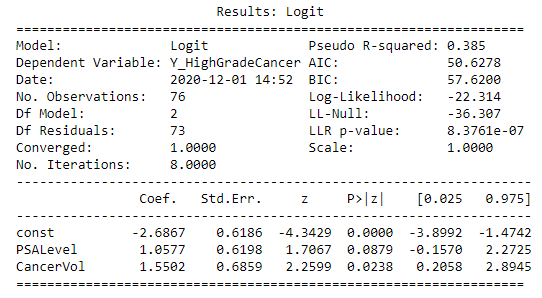
\includegraphics[scale=0.9]{model_fit_python}
	\caption{Maximum Likelihood Estimates of Logistic Regression Function - \textit{Python} Output.}
\end{figure}

Thus, the estimated logistic response function is:

\begin{equation}
\hat{\pi}=[ 1+ exp(-2.6867 + 1.0577X_1 + 1.5502X_2)]^{-1}
\end{equation}

\textbf{Note}: Although the PSALevel predictor is not of 5\% significance (\textit{p}-value=0.0879), I did find it necessary to maintain within this model. When removed, the Residual Deviance score of 44.628 from Figure 4 rose to a value of 48.123. Therefore, I've deemed it a valuable and impactful variable to achieve high model accuracy, and have not removed it from this subset of predictors. \par
With the estimated logistic regression equation now developed, it is left to consider second-order options and make adjustments if required, analyze the residuals and influential observations, test goodness of fit, apply a prediction rule for new observations, and finally apply the final model to the validation data and evaluate the results.

\subsubsection{Geometric Interpretation}
When fitting a standard multiple logistic regression model with two predictors, the estimated regression shape is an S-shaped surface in three-dimensional space. Figure 6 displays a three-dimensional plot of a logistic response function that depicts the relationship between the diagnosis of high grade prostate cancer (\textit{Y}, the binary outcome) and two continuous predictors, PSA Level (\textit{X}\textsubscript{1}) and Cancer Volume (\textit{X}\textsubscript{2}). \par
This surface increases in an approximately linear fashion with increasing values of PSA Level and Cancer Volume, but levels off and is nearly horizontal for very small and large values of these predictors.

\begin{figure}[H]
	\centering
	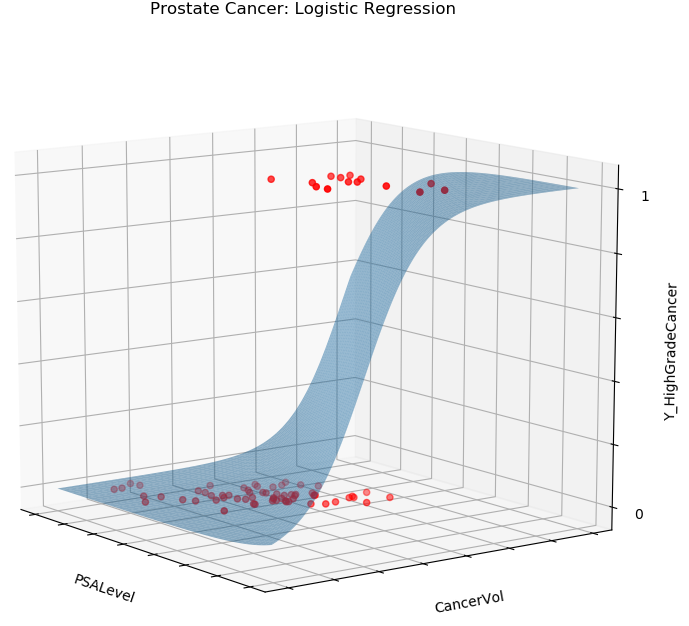
\includegraphics[scale=0.6]{3d_plot}
	\caption{Three-Dimensional Fitted Logistic Response Surface.}
\end{figure}

\subsubsection{Second-Order Predictors}
Occasionally, the first-order logistic model may not provide a sufficient fit to the data, and the inclusion of higher-order predictors may be considered. I'll conclude my model development stage by attempting to fit the Prostate Cancer data to a \textit{polynomial logistic} regression model of the second order, and analyze the results. \par 
For simplicity, a 2\textsuperscript{nd}-order polynomial model in \textit{two} predictors has a logit response function as:

\begin{equation}
logit(\pi) = \beta_0 + \beta_1x_1 + \beta_2x_2 + \beta_{11}x_1^2 + \beta_{22}x_2^2 + \beta_{12}x_1x_2
\end{equation}

\noindent and can be extended to more predictors by the inclusion of additional variables, their coefficients, and accompanying cross terms. Please recall, the Prostate Cancer data set considers 7 predictors. \par
In many situations the true regression function has one or more peaks or valleys, and in such cases a polynomial function can provide a satisfactory approximation. However, a polynomial fit was not successful here, as indicated by \textit{non-significant} p-values across all predictors, at 5\% significance (Figure 7). 

\begin{figure}[H]
	\centering
	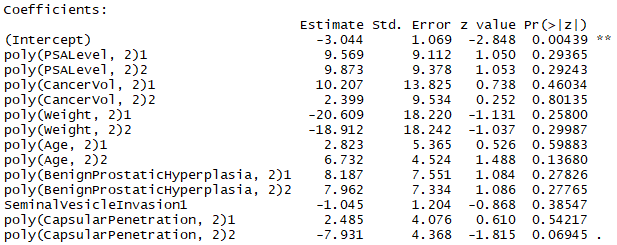
\includegraphics[scale=0.9]{poly_output}
	\caption{Logistic Regression Fit for Second-Order Model - \textbf{R} Output.}
\end{figure}

Additionally, my preliminary scatter plot analysis did not indicate any reason to believe a polynomial fit would be suitable in this study. For example, PSALevel was a major focus of this study and I've provided the scatter plot below in Figure 8 (full data set plotted). Additional scatter plots are provided in the Appendix, \S7.1.

\begin{figure}[H]
	\centering
	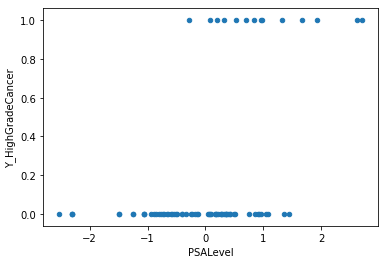
\includegraphics{psalevel_scatterplot}
	\caption{PSALevel vs Y\_HighGradeCancer Scatterplot.}
\end{figure}

Without evidence to be concerned of successfully fitting a model with second-order predictors, I will move forward with my analysis of the previously developed multiple logistic linear regression model.


\subsection{Analysis of Residuals}
In this section I will discuss the analysis of residuals and the identification of any influential observations for logistic regression. Due to the nature of logistic regression, and the fact that non-constant variance is always present in this setting, I will focus only on the detection of model inadequacy.

\subsubsection{Logistic Regression Residuals}
If the logistic regression model is correct, then \(E[Y_i]=\pi_i\) and it follows that:

\begin{equation}
E[Y_i-\hat{\pi}_i]=E[e_i]=0
\end{equation}

This suggests that if the model is correct, a lowess smooth of the plot of residuals against the linear predictor \(\hat{\pi}^{'}_i\) should result in approximately a horizontal line with zero intercept. Any significant departure from this suggests that the model may be inadequate. Shown in Figure 9 are the Pearson residuals plotted against the linear predictor, with the lowess smooth superimposed.

\begin{figure}[H]
	\centering
	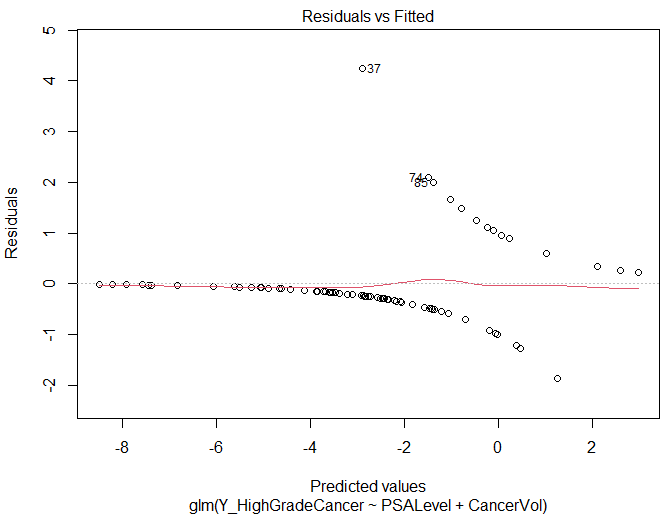
\includegraphics[scale=0.70]{residual_plot}
	\caption{Pearson Residual Plot with Lowess Smooth.}
\end{figure}

Looking at the plot, the lowess smooth adequately approximates a line having zero slope and zero intercept, and I conclude that no significant model inadequacy is apparent. 

\subsubsection{Influential Observations}
To aid in the identification of influential observations, I will use the \textbf{Cook's Distance} statistic, \(D_i\), which measures the standardized change in the linear predictor \(\hat{\pi}_i\) when the \textit{i}th case is deleted. Cook's distances are listed in the \textbf{R} Appendix \S7.2 for a portion of the Prostate Cancer testing data. \par
The plot of distances in Figure 10 identifies observation 90 as being the most outlying in the \textit{X} space, and therefore potentially influential - observations 37 and 91 also read relatively high values. Observation 90 was temporarily deleted and the logistic regression fit was obtained. The results were not particularly different from those obtained from the full test set, and the observation was retained. \textbf{Note}: I additionally and temporarily removed observations 37 and 91 and obtained a fit to the updated final model. The results were not particularly different, and those records were also retained. Thus, no changes to the model are yet necessary.

\begin{figure}[H]
	\centering
	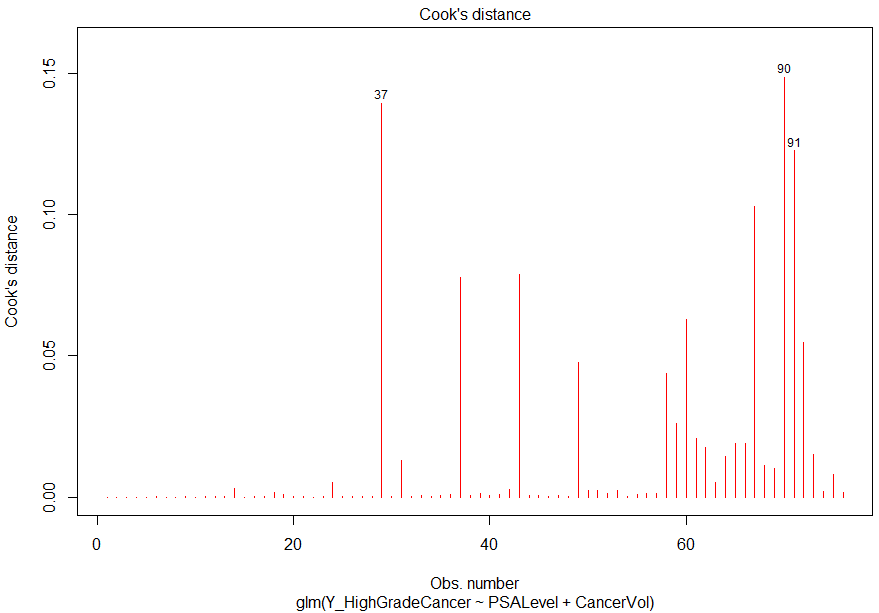
\includegraphics[scale=0.55]{cooks_distance}
	\caption{Index Plot of Cook's Distances.}
\end{figure}


\subsection{Goodness Of Fit Evaluation}
The appropriateness of the fitted logistic regression model needs to be examined before it is accepted for use. In particular, we need to examine whether the estimated response function for the data is monotonic and sigmoidal in shape, as are logistic response functions. Here I will employ the Hosmer-Lemeshow test, which is useful for unreplicated data sets, as is the Prostate Cancer data. The test can detect major departures from a logistic response function, and the alternatives of interest are as follows:

\begin{align}
\begin{split}
	H_0: E[Y]=  [1+exp(-\textbf{X}'\boldsymbol{\beta})]^{-1} \\
	H_1: E[Y] \neq  [1+exp(-\textbf{X}'\boldsymbol{\beta})]^{-1}
\end{split}
\end{align}

\subsubsection{Hosmer-Lemeshow}
The Hosmer-Lemeshow Goodness of Fit procedure consists of grouping that data into classes with similar fitted values \(\hat{\pi}_i\), with approximately the same number of cases in each class. Once the groups are formed, the Hosmer-Lemeshow goodness of fit statistic is calculated by using the Pearson chi-square test statistic of observed and expected frequencies. The test statistic is known to be well approximated by the chi-square distribution with \(c-2\) degrees of freedom.

\begin{equation}
	\chi^2 = \sum_{j=1}^{c} \sum_{k=0}^{1} \frac{(O_{jk}-E_{jk})^2}{E_{jk}}
\end{equation}

The output from \textbf{R} using 5 groups is shown in Figure 11 below.

\begin{figure}[H]
	\centering
	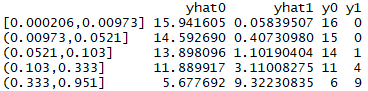
\includegraphics{gof_detail}
	% \caption{insert caption here}
	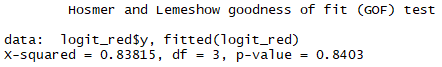
\includegraphics{gof_results}
	\caption{Hosmer-Lemshow Goodness of Fit Test for Logistic Regression Function.}
\end{figure}

Large values of the test statistic X\textsuperscript{2} indicate that the logistic response function is not appropriate. The decision rule for testing the alternatives (Eqn. 10) when controlling the level of significance at \(\alpha\) therefore is:

\begin{align}
\begin{split}
	\textrm{If X\textsuperscript{2}} \leq \chi^2(1-\alpha; c-p)\textrm{, conclude } H_0 \\
	\textrm{If X\textsuperscript{2}} > \chi^2(1-\alpha; c-p)\textrm{, conclude } H_1
\end{split}
\end{align}

Thus, for \(\alpha=0.05\) and \(c-2=5-2=3\), we require \(\chi^2(0.95; 3)=7.81\). Since \(X^2=0.838\leq7.81\), we conclude \textit{H}\textsubscript{0}, that the logistic response function is appropriate. The \textit{p}-value of the test is 0.8403.


\subsection{Development of ROC Curve}
Multiple logistic regression is often employed for making predictions for new observations.
The \textit{receiver operating characteristic} (ROC) \textit{curve} plots \(P(\hat{Y}=1 | Y=1)\) as a function of \(1-P(\hat{Y}=0 | Y=0)\) and is an effective way to graphically display prediction rule information, and possible cutoff points. \par
The "True Positive" \textit{y}-axis on an ROC curve is also known as \textit{sensitivity}, and the "False Positive" \textit{x}-axis is 1-\textit{specificity}. Figure 12 below exhibits the ROC curve for my model (Eqn. 7) for all possible cut points between 0 and 1.

\begin{figure}[H]
	\centering
	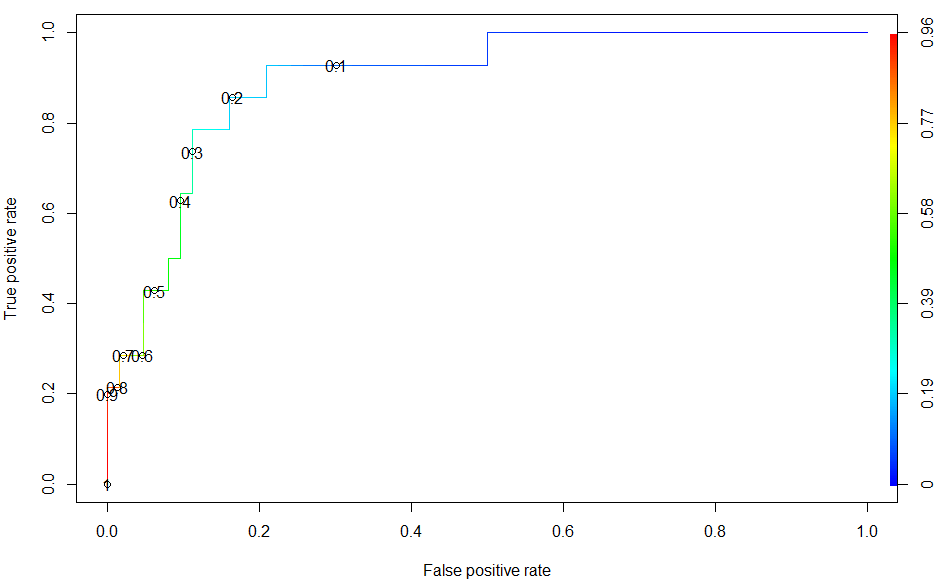
\includegraphics[scale=0.45]{roc}
	\caption{ROC Curve.}
\end{figure}

\subsubsection{Prediction Rule}
In the training data set (which represented a random 80\% of the 97 provided observations), there were 14 men who were observed as high grade cancer patients; hence the estimated proportion of persons who had high grade cancer is \(14/76=0.184\). This proportion can be used as the starting point in the search for the best cutoff in the prediction rule. \par
Thus, if \(\hat{\pi}_h\) represents a newly fitted observation, my first prediction rule investigated is:

\begin{equation}
	\textrm{Predict 1 if } \hat{\pi}_h \geq 0.184\textrm{; predict 0 if } \hat{\pi}_h < 0.184
\end{equation}

The Confusion Matrix of Table 1 below provides a summary of the number of correct and incorrect classifications based on the initial prediction rule (Eqn. 13). Of the 62 men without high grade cancer, 13 would be incorrectly predicted to have high grade cancer, or an error rate of 21.0\%. Furthermore, of the 14 persons with high grade cancer, 1 would be incorrectly predicted with the rule (Eqn. 13) to not have high grade cancer, or 7.1\%. Altogether, \(13+1=14\) of the 76 predictions would be incorrect, so that the prediction error rate for the rule (Eqn. 13) is \(14/76=0.184\) or 18.4\%. Coincidentally, the model exactly matches our training set proportions with the current prediction rule. \par

\begin{table}[H]
	\centering
	\begin{tabular}{ |c||c|c||c|  }
 	\hline
 	\multicolumn{4}{|c|}{Prediction Rule Eqn. 13} \\
 	\hline\hline
 	True Classification&\(\hat{Y}=0\)&\(\hat{Y}=1\)&Total\\
 	\hline
 	\(Y=0\)&49&13&62\\
 	\(Y=1\)&1&13&14\\
 	\hline\hline
 	Total&50&26&76\\
 	\hline
	\end{tabular}
 	\caption{Classification based on Logistic Response Function Eqn. 7 and Prediction Rule Eqn. 13.}
\end{table}

With this baseline understood, it is straightforward to choose a stronger cutoff point in utilizing the ROC curve of Figure 12. As detailed above, the false-positive rate is not ideal at 21.0\% - there are too many cases where a man may opt for additional screening and treatment, even invasive actions, because he believes he has high grade prostate cancer. It will be wise to now reference the ROC curve to better choose a prediction cutoff, while also not significantly disturbing the false-negative accuracy for the worse. \par
Looking at Figure 12 I see a step occurring at 0.20 and use this value for my new cutoff candidate. Thus, my updated prediction rule is stated as follows:

\begin{equation}
	\textrm{Predict 1 if } \hat{\pi}_h \geq 0.20\textrm{; predict 0 if } \hat{\pi}_h < 0.20
\end{equation}

and the effects of this change can be summarized by the Confusion Matrix in Table 2 below.

\begin{table}[H]
	\centering
	\begin{tabular}{ |c||c|c||c| }
 	\hline
 	\multicolumn{4}{|c|}{Prediction Rule Eqn. 14} \\
 	\hline\hline
 	True Classification&\(\hat{Y}=0\)&\(\hat{Y}=1\)&Total\\
 	\hline
 	\(Y=0\)&52&10&62\\
 	\(Y=1\)&2&12&14\\
 	\hline\hline
 	Total&54&226&76\\
 	\hline
	\end{tabular}
 	\caption{Classification based on Logistic Response Function Eqn. 7 and Prediction Rule Eqn. 14.}
\end{table}

The model accuracy has now increased with a significantly better false-positive rate, and intended to reduce financial stress across the healthcare economy.


\subsection{Model: Strengths and Weaknesses}
\subsubsection{Strengths}
-The two predictors which build the final logistic model are PSA Level and Cancer Volume, and they both are adequately correlated with the dependent (outcome) variable Y\_HighGradeCancer - their correlation values are 0.497 and 0.565, respectively. In fact, they are more correlated to the dependent variable than any other predictors of the data set. A consumable heat-map version of a correlation matrix is provided by Figure 13 below, with a color legend given in the upper-left corner.

\begin{figure}[H]
	\centering
	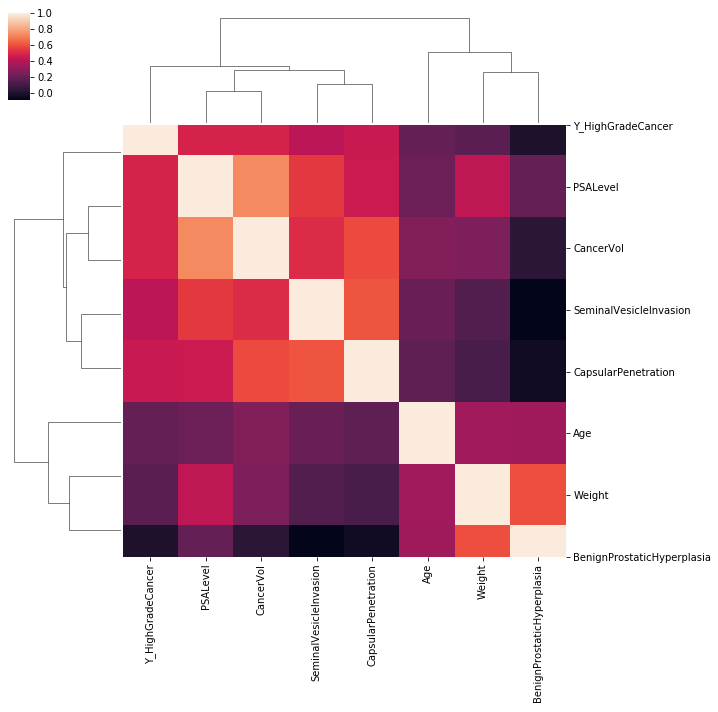
\includegraphics[scale=0.7]{corr_map}
	\caption{Correlation Heatmap - Full Data}
\end{figure}

-The final model has an excellent accuracy score of 84.21\%. Deploying this model in use could help non high grade cancer men be categorized as such, and thus not pursue unnecessary invasive testing and not inflate costs within the healthcare system. Also, by properly identifying those men who are high grade cancer patients, treatment and a plan can be devised sooner, as well as doing so by only use of PSA Level and Cancer Volume information, and not invasive testing. \\ 

\subsubsection{Weaknesses}
-An initial concern while building this model occurs at the level of the provided raw data, namely the existence of multicollinearity. Figure 14 below is the Correlation Matrix of the two final predictors which built the final logistic model: PSA Level and Cancer Volume.

\begin{figure}[H]
	\centering
	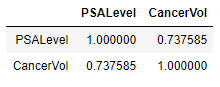
\includegraphics[scale=1.0]{corr_matrix}
	\caption{PSALevel vs. CancerVol Correlation Matrix - Full Data}
\end{figure}

As shown, PSA Level and Cancer Volume have a mild correlation value of 0.624 in the full data set. One primary danger in designing models with multicollinearity is that small changes to the input data can lead to large changes in the model, which can further lead to over-fitting. Therefore, this logistic model may be considered mildly "noisy", sensitive, and not particularly robust. \\

-The Goodness of Fit Evaluation of \S4.4 deserves some concern regarding the Pearson chi-square test. As described previously, the Hosmer-Lemeshow procedure was utilized to determine a goodness of fit, and the test statistic is known to be well approximated by the chi-square distribution with \(c-2\) degrees of freedom (Eqn. 11). However, in view of the \textbf{R} output (Figure 11) with 5 groupings, the expected values (\textit{y\textsubscript{1}}) returned were: 0, 0, 1, 4, 9. Because many values are less than 5, and two of the expected values equal 0, the conditions for a chi-square test may be voided, and it may not be an appropriate test procedure here. At the very lest, the results of the Hosmer-Lemeshow test should be accepted carefully. \\

-The final model may produce high false-negative rates. In view of Figure 15-A we see that the first prediction cutoff of 0.184 produced 1 count of false-negatives (\(7.1\%\) error rate), and an overall model accuracy of \(81.58\%\). After ROC analysis the final prediction cutoff I've employed is 0.20. By Figure 15-B this rule produces 2 counts of false-negatives (\(14.3\%\) error rate), and an overall model accuracy of 84.21\%. Thus the overall model accuracy has improved 2.63 percentage points by correctly predicting more non high grade cancer cases, but has concurrently doubled the false-negative rate. Because correctly identifying high grade cancer patients may be considered most important, this arrangement may be a downfall of the final model.

\begin{figure}[H]
\centering
\begin{subfigure}{.5\textwidth}
  \centering
  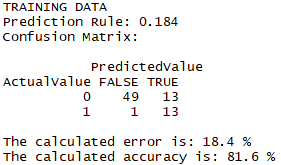
\includegraphics[width=.8\linewidth]{confusion_matrix_PR1}
  \caption{Confusion Matrix - 0.184 Cutoff Rule.}
  \label{fig:sub1}
\end{subfigure}%
\begin{subfigure}{.5\textwidth}
  \centering
  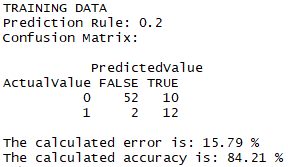
\includegraphics[width=.8\linewidth]{confusion_matrix_PR2}
  \caption{Confusion Matrix - 0.20 Cutoff Rule}
  \label{fig:sub2}
\end{subfigure}
\caption{Classification Based on Logistic Response Function (Eqn. 7) and Prediction Rules (Eqn. 13) and (Eqn. 14).}
\label{fig:test}
\end{figure}